\section{Experiment}
Our setup consists of a glass bulb, connected to a voltmeter used to measure pressure, a pump for evacuating the bulb and a balloon, which is again connected to a bottle filled with helium (see figure 2). 

Our first task is to calibrate the pressure sensor as it outputs just voltage, not pressure directly. For that we need to measure voltages of two known pressures, in our case the air pressure $p_L$ in the lab and the one of near vacuum $p_t$. To evaulate the air pressure there is a mercury barometer available in the lab. First we get the signal $U_L$ from exposing the sensor to air pressure. After that, we evacuate the bulb with the pump and get $U_t$, the voltage at near vacuum (the pump should be able to produce a pressure significantly below \SI{0.2}{\milli\bar}). From those two measurments we can evaluate the slope $C$ and the offset $p_0$ of the so called characteristic curve of the sensor. Now we can translate voltage to pressure with the following formula.

\begin{align}
	p(U) = p_0 + CU
\end{align}


The next step is the experimental part. As said before we want to measure the pressure of a given amount of gas in a constant volume at two different known temperatures. 

The first step is to fill the glass bulb with helium. We want to be sure that there is no air remaining in the bulb, so we evacuate it first, fill it with helium, and then repeat this process. To fill the bulb with helium without too much pressure, we first fill the balloon to around the size of a football and fill the bulb from there, not from the helium bottle directly. We remove the hose at opening 6 before exposing the bulb to heat. Because the pressure in the bulb will increase, air will not get into the bulb. 

We place a water cooker under the bulb with a container, so the bulb will be exposed to the vapor as good as possible. After the voltage has settled we close opening 6, read the signal of the sensor $U_k$ and convert it to pressure $p_k$ with formula (1). We can determine the boiling temperature of water with our measured air pressure and a convesion table. 

Next we place the bulb in a container filled with ice and water. Again, after the voltage signal has settled, we can read $U_e$ and calculate $p_e$.

In the last part of the experiment, we want to use our setup as a gas thermometer and measure the temperature of liquid nitrogen. For that we completly submerge the bulb as it is in a container of liquid nitrogen, read the voltage $U_n$ and calculate $p_n$.

\begin{figure}[h]
	\centering
	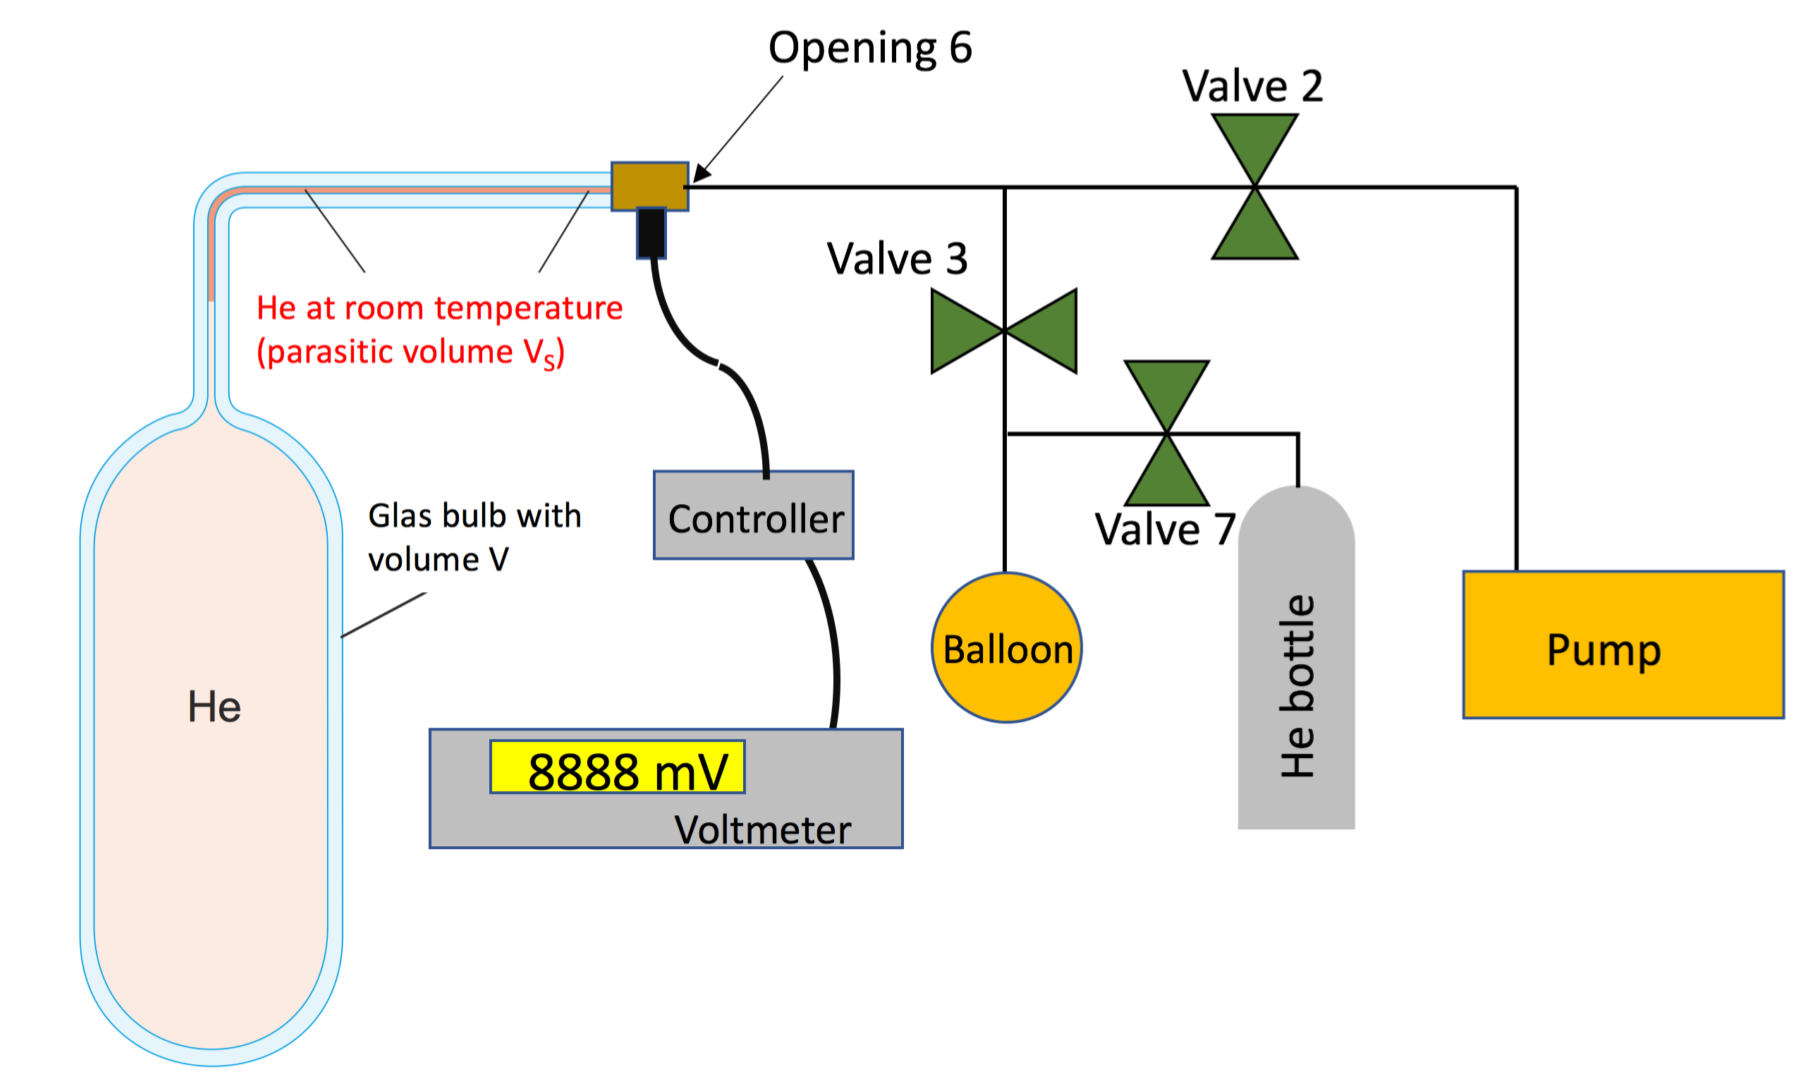
\includegraphics[width=0.5\textwidth]{sections/images/schematic.png}
	\caption{Schematic taken from the experiment manual}
\end{figure}
